% Exposition on Emotiq Crypto
% DM/Emotiq  02/18
%
\documentclass[article,oneside]{memoir}
\usepackage{geometry} 
\geometry{letterpaper} 
%\usepackage[parfill]{parskip}    % Activate to begin paragraphs with an empty line
\usepackage{graphicx}
\usepackage{amsmath}
\usepackage{amssymb}
\usepackage{epstopdf}
\usepackage[latin1]{inputenc}
\usepackage{fancyhdr}
\usepackage{dcolumn}
\usepackage[pdftex,bookmarks]{hyperref}
\usepackage{moreverb}
\usepackage{listings}

\DeclareGraphicsRule{.tif}{png}{.png}{`convert #1 `dirname #1`/`basename #1 .tif`.png}

% \usepackage[draft]{pdfdraftcopy}
% \draftstring{PRELIMINARY}
% \definecolor{my-draft-color}{rgb}{0.85,0.85,0.85}
% \draftcolor{my-draft-color}
%      \watermarkgraphic{/usr/local/lib/Logo75Img-Alpha25y.pdf}
% \watermark


%% -----------------------------------------------------------------------------------------------------------------------
\pagestyle{fancy}
\fancyhf{}  %delete current header and footer
\fancyhead[L]{\bfseries{Emotiq Crypto Features}}
\fancyhead[R]{\bfseries\thepage}
\fancyfoot[L]{\small{Copyright {\copyright} 2018 by Emotiq AG}}
\renewcommand{\headrulewidth}{0.5pt}
\renewcommand{\footrulewidth}{0.5pt}
\addtolength{\headheight}{0.5pt} % space for the rule

%\fancypagestyle{plain}{%
%	\fancyhead{} % get rid of headers on plain pages
%	\renewcommand{\headrulewidth}{0pt} % and the line
%	}
	
%% -----------------------------------------------------------------------------------------------------------------------
\title{Emotiq Crypto Features}
\author{David McClain, Emotiq AG\\dbm@emotiq.ch\\1st Draft}
%\date{\today}  % leave commented out for current date to show
%\date{Friday, June 15, 2007}

\begin{document}
\maketitle

\tableofcontents*

%% -----------------------------------------------------------------------------------------------------------------------
%% Our Commentary

%%%%%%%%%%%%%%%%%%%%%%%%%%%%%%%%%%%%%%%%%%%%%%%
\lstset{ %
language=Lisp,                % choose the language of the code
basicstyle=\footnotesize,       % the size of the fonts that are used for the code
numbers=left,                   % where to put the line-numbers
numberstyle=\footnotesize,      % the size of the fonts that are used for the line-numbers
stepnumber=2,                   % the step between two line-numbers. If it's 1 each line will be numbered
numbersep=5pt,                  % how far the line-numbers are from the code
backgroundcolor=\color{white},  % choose the background color. You must add \usepackage{color}
showspaces=false,               % show spaces adding particular underscores
showstringspaces=false,         % underline spaces within strings
showtabs=false,                 % show tabs within strings adding particular underscores
frame=single,	                % adds a frame around the code
tabsize=2,	                % sets default tabsize to 2 spaces
captionpos=b,                   % sets the caption-position to bottom
breaklines=true,                % sets automatic line breaking
breakatwhitespace=false,        % sets if automatic breaks should only happen at whitespace
escapeinside={\%*}{*)}          % if you want to add a comment within your code
}

%%%%%%%%%%%%%%%%%%%%%%%%%%%%%%%%%%%%%%%%%%%%%%%

\chapter{Pairing-based Cryptography}

Emotiq utilizes advanced bilinear pairing-based cryptography\cite{thesis}\cite{lib} (PBC) for user keying, Boneh-Lynn-Shacham (BLS) Signatures\cite{bls}, fast multi-party signatures, and for Randomness Generation. The advantages of PBC are numerous and include short signatures, fast signature generation, safe deterministic hierarchical wallet keying, and fast multiparty randomness generation.

A bilinear pairing uses pairs of Elliptic Curves, defined over two separate groups, such that their bilinear mappings produce homomorphic encryption in a resulting composite field. If we denote the two curve groups as $G1$ and $G2$,  their pairing field $GT$, and prime order finite field $Zr$, then their pairing $e(G1,G2) \in GT$ is such that $$e(a U, V) = e(U, a V)= g^a$$ where $U \in G1$, $V \in G2$, $a \in Zr$, and $g \in GT$.

In our system group $G1$ is always the smaller group, with the shortest representation. Specifically, our $Zr$ uses 256 bits, $G1$ was chosen to have a 264-bit representation, $G2$ has a 520-bit representation, $GT$ has a 3072-bit representation, and the prime order of the groups is $q \approx  2^{254}$, which gives us roughly $2^{127}$ security.

Private keys belong to the finite field $Zr$ with the same prime group order. Public keys are generated in $G2$, and signatures are generated in $G1$. The embedding degree of our curves is 12, and correspond to {\emph{Type f}} asymmetric pairing curves in Lynn's Thesis\cite{thesis}. Wherever they occur, we use  compressed point representation for group elements from $G1$ and $G2$.

The complete specification of the Emotiq cryptosystem requires knowledge of all curve pairing parameters, plus two chosen generators $U \in G1$, and $V \in G2$.

\chapter{Boneh-Lynn-Shacham (BLS) Signatures}

BLS signatures are the shortest possible, and enable multisignature generation in just one pass. A BLS signature on message $msg$ is computed as $$sig = s G1(H(msg))$$ where $H(x)$ is the SHA3/256 hash of its argument, $s \in Zr$ is the user's secret key value, and $G1(H(x)) \in G1$ is the group member that corresponds to that hash value. A signature is always accompanied by the public key of the signer, $P = s V$, for generator $V \in G2$,  producing a signed message as a triple $$(msg, sig, P)$$

Because of homomorphism we can verify a signature by noting that a valid signature exhibits the pairing relationship $$e(s  G1(H(msg)),V) = e(G1(H(msg)), s V) = e(G1(H(msg)), P)$$

And also because of homomorphism, we can easily compute a multi-party signature by simply summing the individual signatures and also summing their corresponding public keys: $$e({\sum_i s_i} G1(H(msg)),V) = e(G1(H(msg)), {\sum_i P_i})$$ producing the collective triple $$(msg, {\sum_i sig_i}, {\sum_i P_i})$$

Therefore, during the computation of collective signatures, we need only a single pass through all participants as we gather and sum their signture components. A collective signature appears no different than a single signature.

In contrast, conventional Schnorr signatures require two signature values, forming a quadruple with message and public key. For message $msg$ the Schnorr signature is the pair $(R,u)$ of an Elliptic Curve point $R$ and a field value $u$, where $R = r G$, for generator point $G$, and $r = H(k_{rand}, msg, P)$ is chosen as a random offset. Finally $u = r + H(R,P,msg) s$. The Schnorr signature is validated by checking that $$u G = R + H(R, P, msg) P$$

For collective Schnorr signing, all participants are asked to compute their own commitments $R_i = r_i G$. Those values are collected and summed to produce a global challenge value, $c_{glb} = H(\sum_i R_i, \sum_i P_i, msg)$.  Then the participants are asked to produce their $u_i$ values against that global challenge:

$$u_i = r_i + c_{glb} s$$

and again the values are summed. Hence collective Schnorr signatures require two interactions with every signer of the message. Network traffic is approximately twice that required for BLS signatures, with a consequent window of opportunity for attackers to spoil the process during the second round.

\chapter{Fast Randomness Generation with PVSS}

The use of BLS Signatures allows an abbreviated form of PVSS randomness generation. Participants in randomness generation are given a list of neighboring group nodes in the network, with whom they carry out a pBFT protocol with publicly verifiable secret sharing (PVSS). 

Within each group, a sharing threshold is set at $t = \lfloor \frac{N}{3} \rfloor + 1$ for group size $N$. Secret random seeds are generated by each participant, then encrypted shares are formed over that secret and distributed to other group members, along with cryptographic proofs on the shares.

For sharing threshold $t$, a random polynomial of order $t-1$ is generated $$p(x) = a_0 + a_1 x + ... + a_{t-1} x^{t-1}$$ with the secret value denoted by $a_0$.  Shares are constructed by computing the value of this polynomial for each member of the group, assigned successive ordinal values, $i = 1 ... N$. The resulting share values, $p(i)$, are then encrypted by multiplying the share value by the public key of each member, $E(share_i) = Zr(p(i)) P_i \in G2$, and proofs are generated by forming a point, $proof_i = Zr(p(i)) U \in G1$, for generator $U \in G1$. 

A vector of shares and a vector of proofs is generated, one element for each member of the group, and these vectors are then transmitted to each group member.
$$(E(share_1), E(share_2), ..., E(share_N))$$
$$ (proof_1, proof_2, ..., proof_N)$$

As with any BLS signature, each share is validated against its proof by checking that the pairings match:
$$ e(proof_i, P_i) = e(U, E(share_i))$$

Every member of the group can also verify that all shares from another group member were consistently generated from the same sharing polynomial. To do so, we treat the share vector as a codeword from a Reed-Solomon encoding\cite{scrape}, compute a random polynomial of order $N - t - 1$ and use that to compute a test vector from the dual-space of the original share generating polynomial:
$$f(x) = b_0 + b_1 x + ... + b_{N-t-1} x^{N-t-1}$$
$$c_{\perp} = (\lambda_1 f(1), \lambda_2 f(2), ... , \lambda_N f(N))$$
where weights $\lambda_i = \prod_{j \ne i} \frac{1}{i-j}$, for $ i,j = 1...N$.
Then the consistency of the encrypted shares is verified by checking that:
$$\sum_i {c_{\perp}}_i proof_i = G1(0)$$

This consistency check is absolutely certain for valid sharing vectors, and has an inconsequential probability of failing to detect an improper sharing set given as $\approx 1/q$, or about 1 chance in $2^{254}$. There is a greater likelihood of finding a hash collision in SHA3/256 than in seeing a failure to detect an inconsistent sharing vector.

After performing consistency checks on the sharing set from one group member, the share directed at one node can be decrypted with its secret key to produce a decrypted share, $$G2(share_i) = \frac{1}{s_i}E(share_i) \in G2$$ for secret key $s_i \in Zr$.

This decrypted share is then broadcast to all group members. Decrypted shares can be verified from the pairing relation:
$$ e(proof_i, V) = e(U, G2(share_i))$$

As soon as a sharing threshold number, $(n \ge t)$, of decrypted shares has been seen for any one sharing set, the secret randomness from that set can be discovered via Lagrange interpolation:
$$G2(random) = \sum_i G2(share_i) \prod_{j \ne i} \frac{i}{i-j}$$

Finally, after a supermajority of sharing sets has been decrypted, $(n \ge 2 \lfloor \frac{N}{3} \rfloor + 1)$, their randomness is combined as a simple sum in $G2$, and forwarded to all other groups.
$$G2(random_{grp}) = \sum_i G2(random_i)$$

Proof of group randomness comes from the sum of Lagrange interpolations of the individual proof sets.
Final randomness results from a supermajority sum of randomness obtained from each group, and its proof results from the sum of group proofs. 

So the use of pairing-based cryptography shows great benefits, not only in minimizing network traffic, and by making immediate commitments to portions along the way, and also from the fact that proofs are so easily generated as simple sums of existing proofs.

Timing tests show that this approach scales linearly with number of group participants, ranging from about 5 seconds for 32 group members, to about 7 minutes for 1024 group members, on an ordinary iMac with an Intel i7 processor. The timings are dominated by compute load, not network communications.

\begin{figure}[h!]
  \centering
  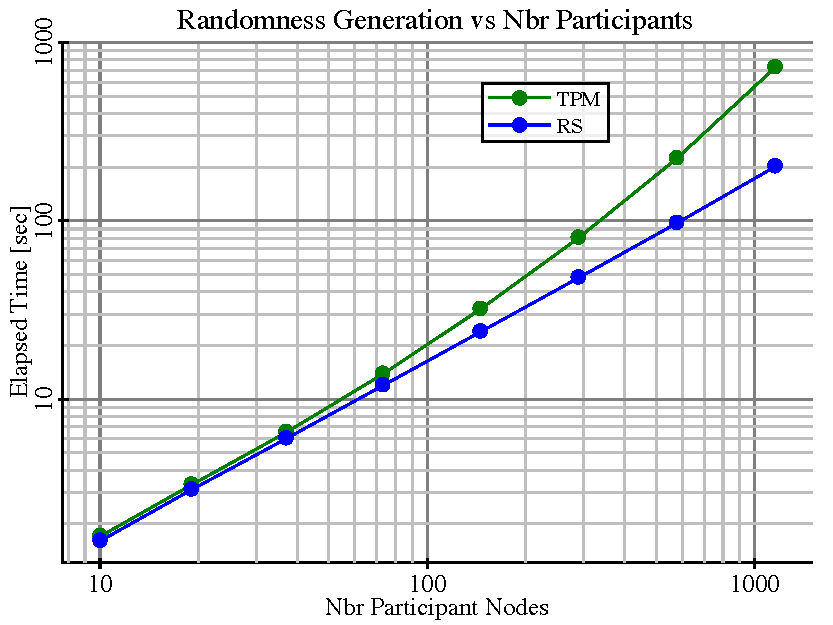
\includegraphics[width=4in]{randtimings}
  \caption{ Comparison of performance between the TPM Method and the Reed-Solomon interpretation of proof vectors.}
  \label{fig:randtimings}
\end{figure}

\chapter{Alternative Method for Randomness Generation}
There is an alternative method for generating randomness with PVSS, which I call the TPM Method.\cite{tpm}\footnote{The paper has an error in that it specifies that encrypted shares should be formed as the product of the share value and the generator of the curve. That is incorrect, as the encryption needs to incorporate information about the target node keying. It seems likely that the error crept in by way of fractured translation to English. I found the nomenclature terribly inconsistent and confusing.} It performs the same share generation procedure as seen above, but instead of sending along a vector of proofs on each encrypted share, it sends along proofs on the sharing polynomial coefficients, $a_i, i = 0..t-1$ using $aproof_i = a_i U$ for generator $U \in G1$.

Then, at each receiving node, the shares are verified by computing the sums
$$ proof_i = \sum_{j=0..t-1} i^j aproof_j, i = 1..N$$
Then the pairing relation is checked
$$e(proof_i, P_i) = e(U,E(share_i))$$

These proof sums correspond directly to the proofs presented in the previous section. And they also directly verify that every encrypted share came from the same polynomial. One advantage of this method is that instead of transmitting $2 N$ vector elements, we now only need to transmit $N+t$ elements.

However, we now also need to supply these proof sums along with any decrypted shares that we compute, and the method scales super-linearly. Timing tests have shown it to be a hair slower than the first method for $N=32$, and about half as fast when $N=1024$. But the method is equivalent in its information content, and every bit as secure.

\chapter{Verifiable Random Functions}
A verifiable random function (VRF)\cite{vrf2} uses a pseudo-random function (PRF) in such a way as to furnish proof that the result was fed a specific seed value to produce the pseudo-random result. We follow the work of Dodis and Yampolskiy\cite{vrf}, to provide a PRF as follows:

For arbitrary input seeding values, form the hash $H(seed)$ using SHA3/256. This converts arbitrary objects of any length into a 256-bit random-like, but reproducible, pattern. Then map that hash value into our $Zr$ field, which has dimension $q = |Zr| \approx 2^{254}$, to produce $x = Zr(H(seed))$.

Output of the VRF is a pseudo-random value in the pairing field (3072 bits) $$y = VRF(s, x) = e(U,V)^{1/(x + s)} \in GT$$ for secret key $s \in Zr$,  generators $U \in G1$, $V \in G2$, and with proof $$R = \frac{1}{x+s}U \in G1$$ 

Output of the VRF is the quadruple $(seed, x, y, R)$, i.e., the original seed, the seed deterministically reduced to an element of $Zr$, the output of the VRF computation, and the point in $G1$ that represents the proof.

Verification of proof checks the pairing $$e(R, x V + P) = e(U,V)  \in GT$$ for public key $P = s V \in G2$, and to verify that $$y = e(R,V)$$ and that $$x = Zr(H(seed))$$

\chapter{Cosi Multisignatures}
We use Cosi trees\cite{cosi} to provide scalable, distributed, multisignature generation. Validator nodes are selected from among a group of stakeholder nodes, using random sortition to assign $N$ of them to a position in a Cosi tree. 

A Cosi tree is an n-way tree, where each node in the tree interior is a group leader over $n$ subnodes, each of which may be group leaders over their own subtrees. At any one time, there may be several Cosi trees operating for different purposes, and some nodes might belong to more than one Cosi tree.

When a signature is requested from a Cosi tree, the message is distributed down through the tree to all participant nodes. Each node then attempts to validate the message and decides whether or not to add its signature to the collective signature formed from the sum of all signatures of its subgroup, before passing the augmented signature back up to its parent node in the tree. Accompanying that signature is a composite public key consisting of the sum of participant node public keys, and a bitmap that represents which nodes actually signed the message.

Validation of a message requires varying computation based on the type of message. For randomness generation, it means validating all publicly verifiable quantities and producing decrypted shares. For block validation it means verifying the public keys of all signers of the block, validating all transactions, and so on.

At the top of the tree the bitmap is converted into a list of public keys for all participating nodes, which is used to verify the summed public key, and to gain a census count on how many nodes actually signed the message. That census count is checked against a pBFT threshold of $2 f+ 2$, where $f = \lfloor \frac{N-2}{3} \rfloor$ is the tolerance for Byzantine failures among the nodes, to decide whether the multisignature is acceptable. 

\chapter{XX}

\chapter{Safe Hierarchical Keying}

In current blockchain designs which utilize simple Elliptic Curve cryptography, the possibility of producing subkeys from a master public key is presented. But that is wholly unsafe in the event that a decryption key is also generated for a derived public key. A simple bit of finite field arithmetic is all it takes to discover the original master private key.

With PBC we can safely generate both public and private keys without exposing our master private key. This is also known as Identity-Based Encryption (IBE). But unlike conventional presentations of IBE, we do not rely on a trusted third party for the generation of our keying. Rather, we view the master key holder as the only entity that should be entitled to generate new decryption keys. 

Anyone can generate new public keys at any time, based on previously known public keys.
But in order to obtain a decryption key for the new public keys, you must ask the primary secret key holder for a decryption key. Doing so puts the primary key holder at no risk for exposing his or her private key.

A new public key can be generated by asking for a subkey of a given public key, using an arbitrary identity value to identify that subkey. The new public key is computed as $$ P_{id} = Zr(H(id)) V + P$$ for identity $id$, generator $V \in G2$, public key $P \in G2$, and where $Zr(H(id)) \in Zr$ is the element of the field that corresponds to the hash of the supplied identity. 

You can use this public key to encrypt a message by making use of the hash of a pairing value as an XOR mask against a message $$E(msg) = msg \oplus H(g^r)$$ where $r = Zr(H(msg, id)) \in Zr$, and pairing element $g^r = e(U, r V)$, for generator $U \in G1$, generator $V \in G2$. The message is transmitted as the triple $(E(msg), R, id)$, with $R = r P_{id} \in G2$.

In order to produce a decryption key for that new public key, the primary key holder computes $$S_{id} = \frac{1}{s + Zr(H(id))} U \in G1$$ for secret key $s \in Zr$. Producing a decryption key in $G1$ ensures, by difficulty of ECDLP, that our master private key remains safe against exposure.

Homomorphism allows us to see that the pairings 
$$e(S_{id}, R) = e(\frac{1}{s + Zr(H(id))} U, r(Zr(H(id)) V + P)) = e(U, r V) = g^r$$ which allows us to recreate the XOR mask and decrypt to the original message $$msg = E(msg) \oplus H(g^r)$$ Verification of the message is done by computing $r = Zr(H(msg, id))$ and checking that $$r (Zr(H(id)) V + P) = R \in G2$$

In this form, a new private key cannot be used to sign messages in the same manner as for BLS signatures with the master private key. But it does furnish a way to encrypt and decrypt messages by using the hash of the pairing result. This technique has been dubbed SAKKE by its authors Sakai-Kasahara\cite{sakke}. We have extended SAKKE encryption to indefinite length by using successive SHA3 hashes on the pairing field result and an increasing index value.

\begin{thebibliography}{99}
%[ ... TBD: fill out the bibliography ... ]

\bibitem{scrape}Ignacio Casudo and Bernardo David, {\em{ SCRAPE: Scalable Randomness Attested by Public Entities}} 
\bibitem{vrf}Yevgeniy Dodis and Aleksandr Yampolskiy, {\em{A Verifiable Random Function With Short Proofs and Keys}}
\bibitem{thesis} Ben Lynn, PhD Thesis, {\em{On the Implementation of Pairing-Based Cryptosystems}}, June 2007
\bibitem{lib} Ben Lynn, PBC Library, https://crypto.stanford.edu/pbc/download.html
\bibitem{bls} Ben Lynn, {\em{BLS Signatures}}, https://crypto.stanford.edu/pbc/manual/ch02s01.html
\bibitem{vrf2}Silvio Micali, Michael Rabin, Salil Vadhan, {\em{Verifiable Random Functions}}
\bibitem{sakke}Sakai-Kasahara, {\em{IETF RFC 6508 Sakai-Kasahara Key Encryption (SAKKE)}} 
\bibitem{cosi}Ewa Syta, Iulia Tamas, Dylan Visher, David Isaac Wolinsky, Philipp Jovanovic, Linus Gasser, Nicolas Gailly, Ismail Khoffi, Bryan Ford, {\em{Keeping Authorities ``Honest or Bust'' with Decentralized Witness Cosigning}}
\bibitem{randhound} Ewa Syta, Philipp Jovanovic, Eleftherios Kokoris Kogias, Nocals Gailly, Linus Gasser, Ismail Khoffi, Michael J. Fisher, Bryan Ford, {\em{Scalable Bias-Resistant Distributed Randomness}}
\bibitem{tpm} Youlian Tian, Changgen Peng, Jianfeng Ma, {\em{Publicly Verifiable Secret Sharing Scheme Using Bilinear Pairings}} 
\end{thebibliography} 

\end{document}
%=%=%=%=%=%=%=%=%=%=%=%=%=%=%=%=%=%=%=%=%=%=%=%=%=%=%=%
